\graphicspath{{images/act_1.2/}}
\subsection{Generate step reference}
\label{subsec:generate_step_reference}
The objective of this activity is to generate a step reference trajectory on the $z$-axis after $2$ seconds of simulation. Likewise, reference trajectory should start in position $p_0=\begin{bmatrix}  0.5765 &   0.1915 &   0.3637 \end{bmatrix}$~m. For this purpose, Algorithm \ref{lst:step_reference_generator} describes a function to generate a step trajectory that consider initial end-effector position. Finally, Figure \ref{fig:act_1.2_step_reference} shows the step reference trajectories that robot end-effector will track in next activities. \vspace{.5cm}

\begin{lstlisting}[language=Python,caption=Function to generate a step reference trajectory., label={lst:step_reference_generator}]
def step_reference_generator(q0, a, t_step, t):
    """
    @info: generate a constant reference.

    @inputs:
    ------
        - q0: initial joint/cartesian position
        - a: constant reference
        - t_step: start step [sec]
        - t: simulation time [sec]
    @outputs:
    -------
        - q, dq, ddq: joint/carteisan position, velocity and acceleration
    """
    if t>=t_step:
        q = q0 + a  # [rad]
        dq = 0      # [rad/s]
        ddq = 0     # [rad/s^2]
    else:
        q = copy(q0)    # [rad]
        dq = 0          # [rad/s]
        ddq = 0         # [rad/s^2]            
    return q, dq, ddq
\end{lstlisting}

\vspace*{0cm}
\begin{figure}
	\centering
	\subfloat[]{
	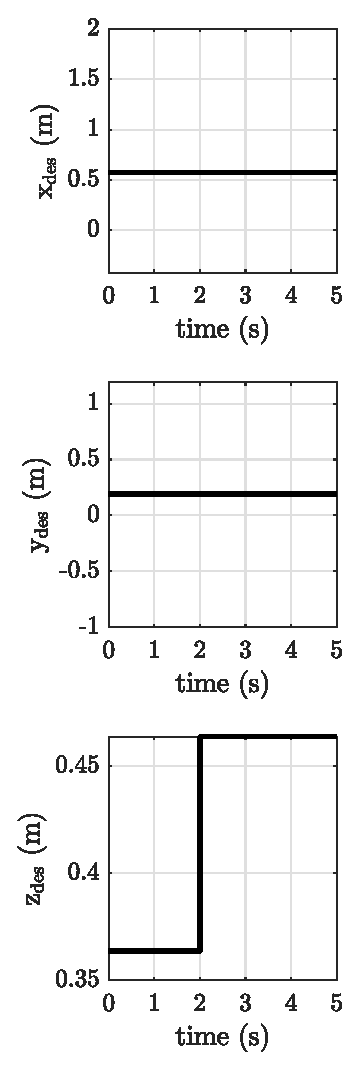
\includegraphics{ee_position.eps}
	%\caption{Reference position for the robot end-effector with Algorithm \ref{lst:sine_reference_generator}.}
	%\label{fig:act_1.1_ee_position}
	}
	\hfill
	\subfloat[]{
	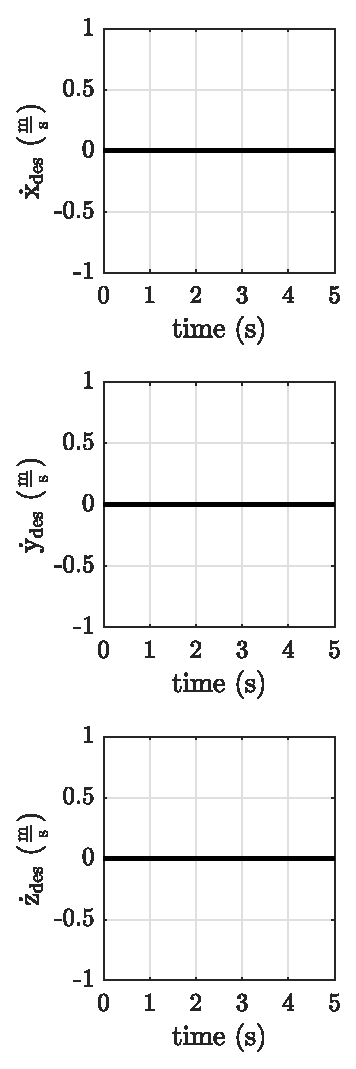
\includegraphics{ee_velocity.eps}
	%\caption{Reference velocity for the robot end-effector with Algorithm \ref{lst:sine_reference_generator}.}
	%\label{fig:act_1.1_ee_velocity}	
	}	
	\hfill
	\subfloat[]{
	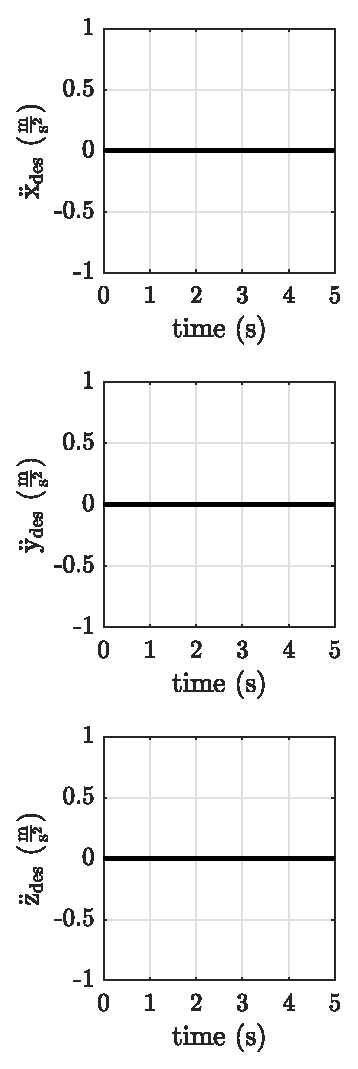
\includegraphics{ee_acceleration.eps}
	%\caption{Reference velocity for the robot end-effector with Algorithm \ref{lst:sine_reference_generator}.}
	%\label{fig:act_1.1_ee_acceleration}	
	}		
	\caption{Cartesian reference trajectories for the robot end-effector with Algorithm~\ref{lst:step_reference_generator}: (a) position, (b) velocity and (c) acceleration.}
	\label{fig:act_1.2_step_reference}
\end{figure}
